\section{Experimental Results}\label{experiments}
% on Correlation Patterns and Analysis
%Findings - reveal correlation of speed and mobile data access

\begin{figure*}
    \centering
		\subfigure[Speed Estimates Empirical CDF\label{fig:speed_cdf}]{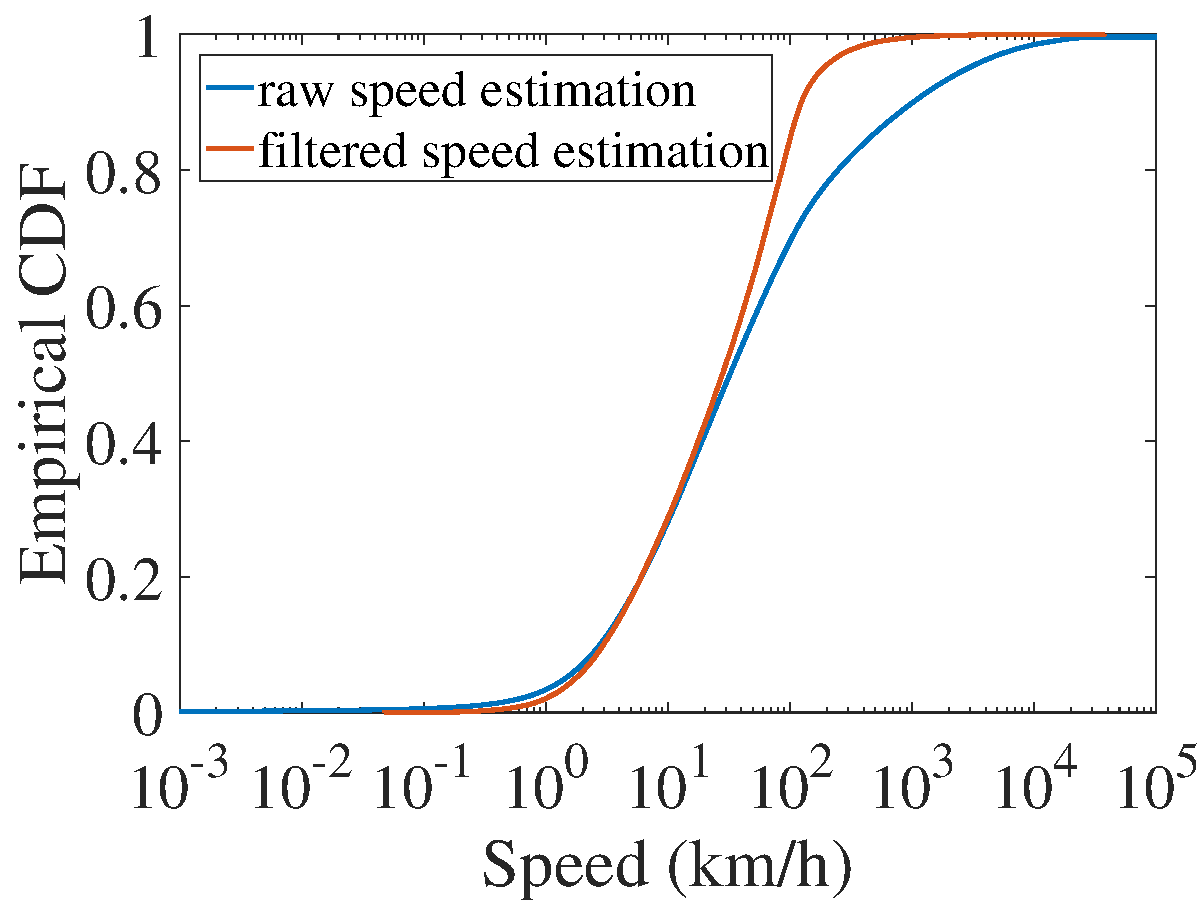
\includegraphics[width=0.32\linewidth]{./figures/large_font/speed_cdf.pdf}}
		\subfigure[Data Volume\label{fig:speed_vol}]{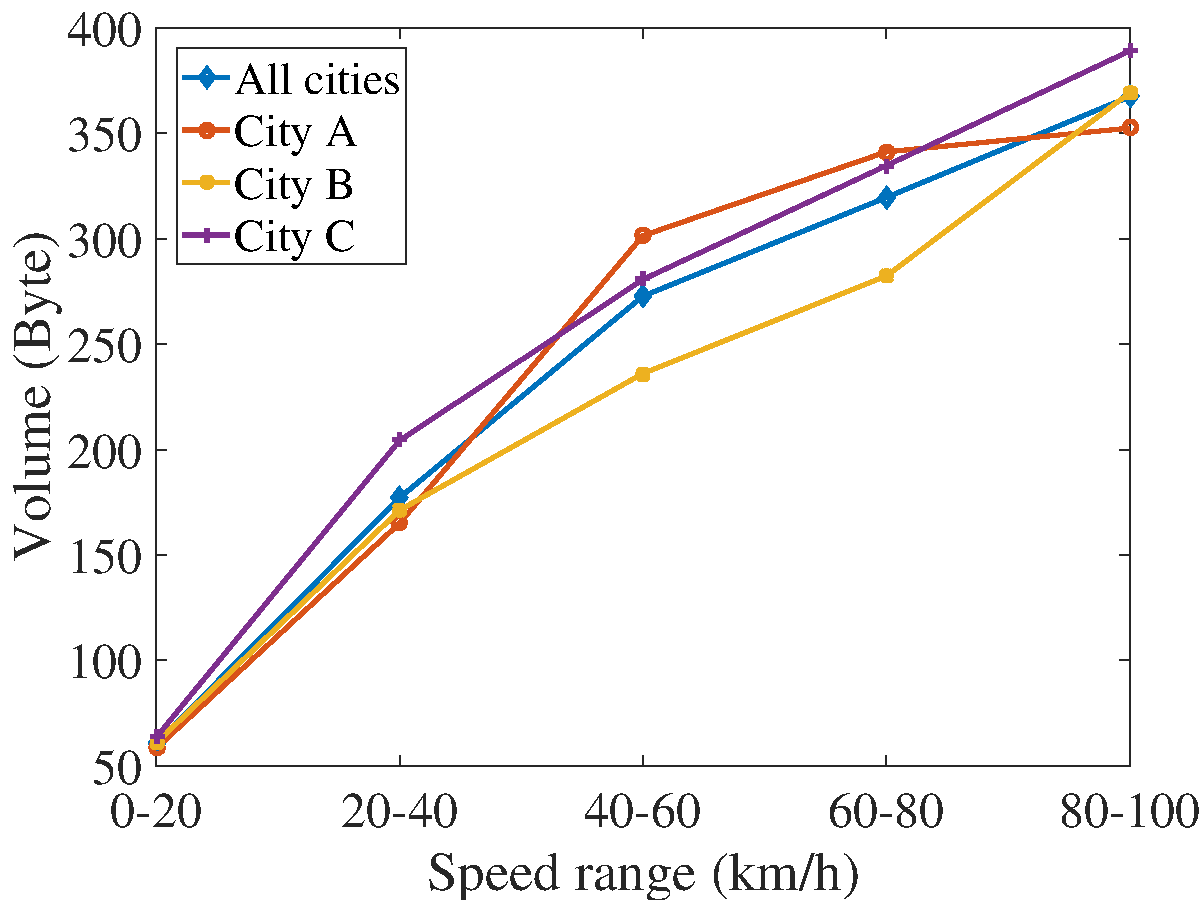
\includegraphics[width=0.32\linewidth]{./figures/large_font/speed_vol.pdf}}
    \subfigure[Average Time Interval\label{fig:speed_gap}]{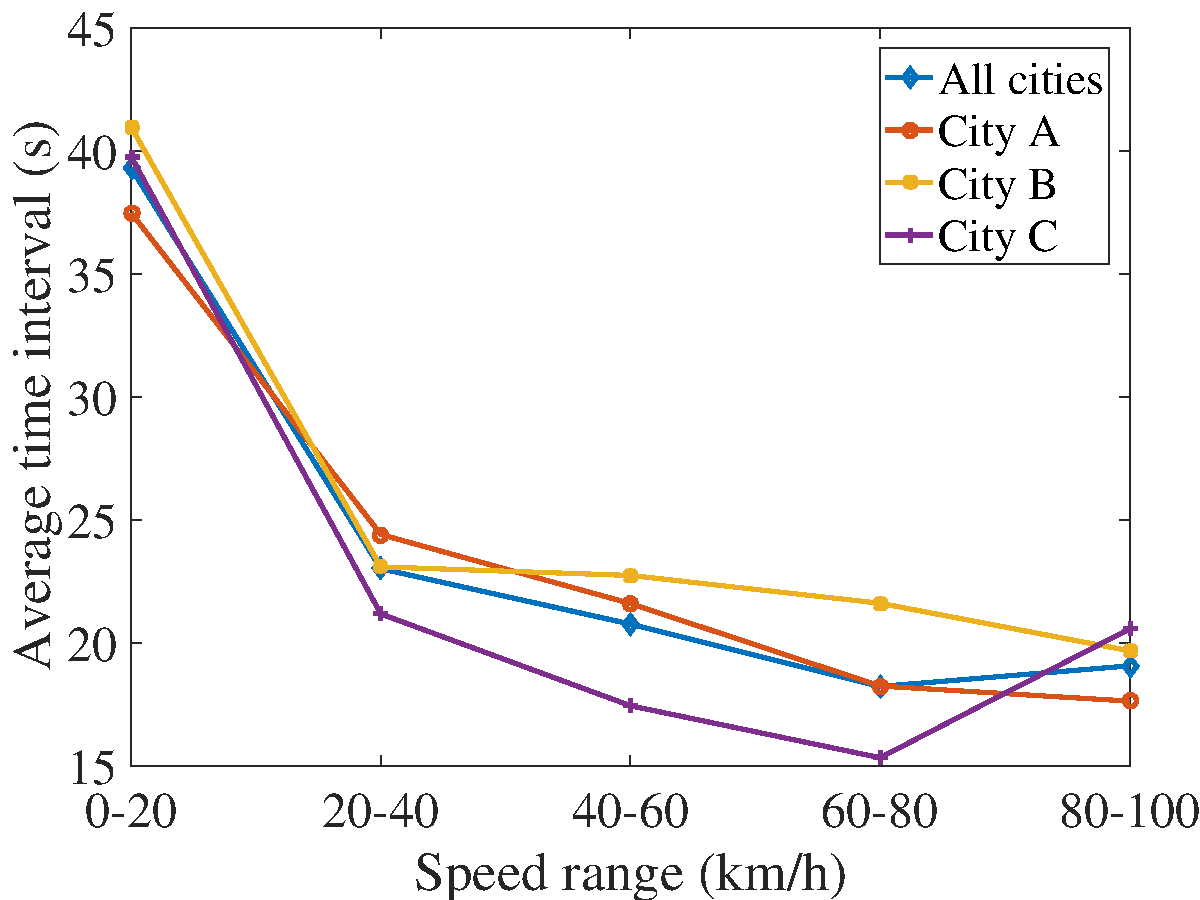
\includegraphics[width=0.32\linewidth]{./figures/large_font/speed_gap.pdf}}
		\subfigure[Time Interval Empirical CDF\label{fig:speed_gap_cdf}]{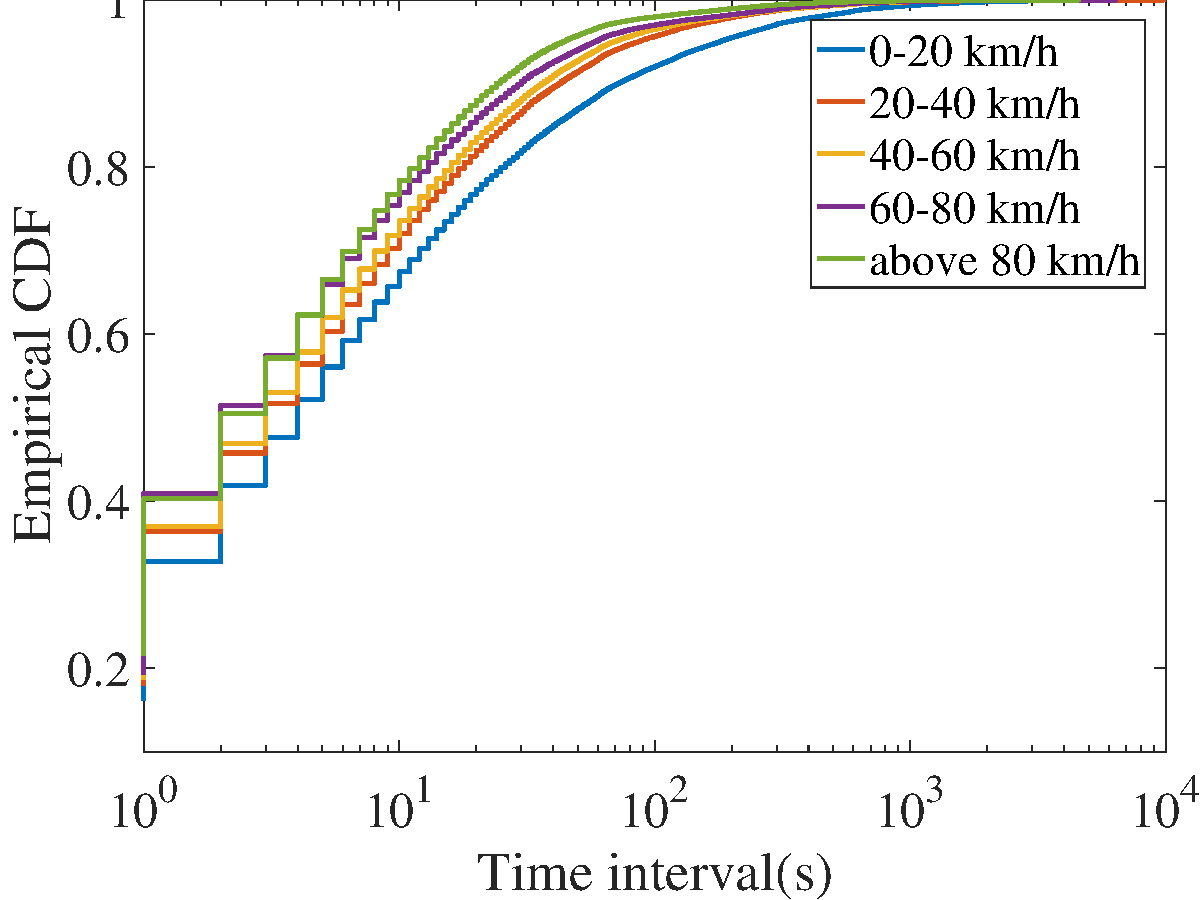
\includegraphics[width=0.32\linewidth]{./figures/large_font/speed_gap_cdf.pdf}}
		\subfigure[Average Volume per Data Access\label{fig:speed_per_conn_vol}]{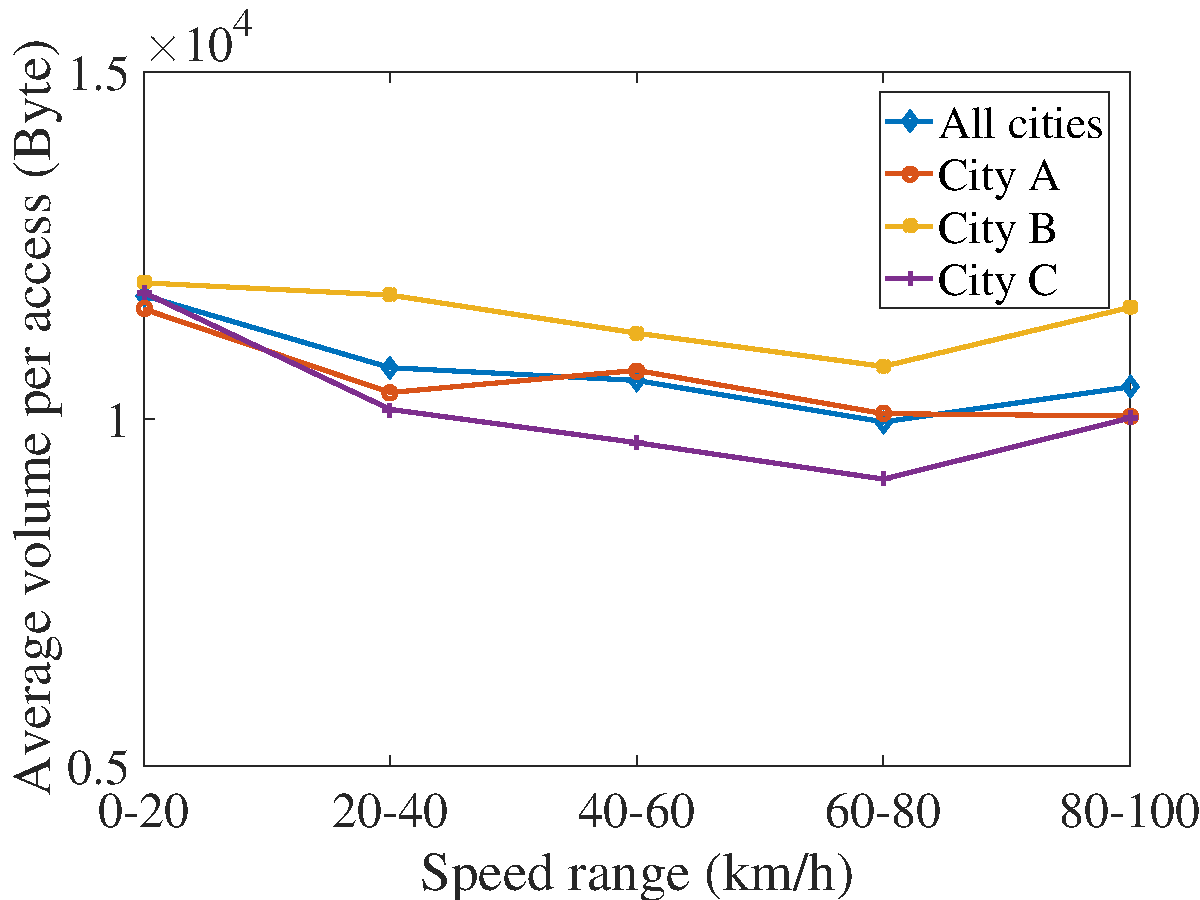
\includegraphics[width=0.32\linewidth]{./figures/large_font/speed_per_conn_vol.pdf}}
		\subfigure[Number of Apps Used\label{fig:speed_diversity}]{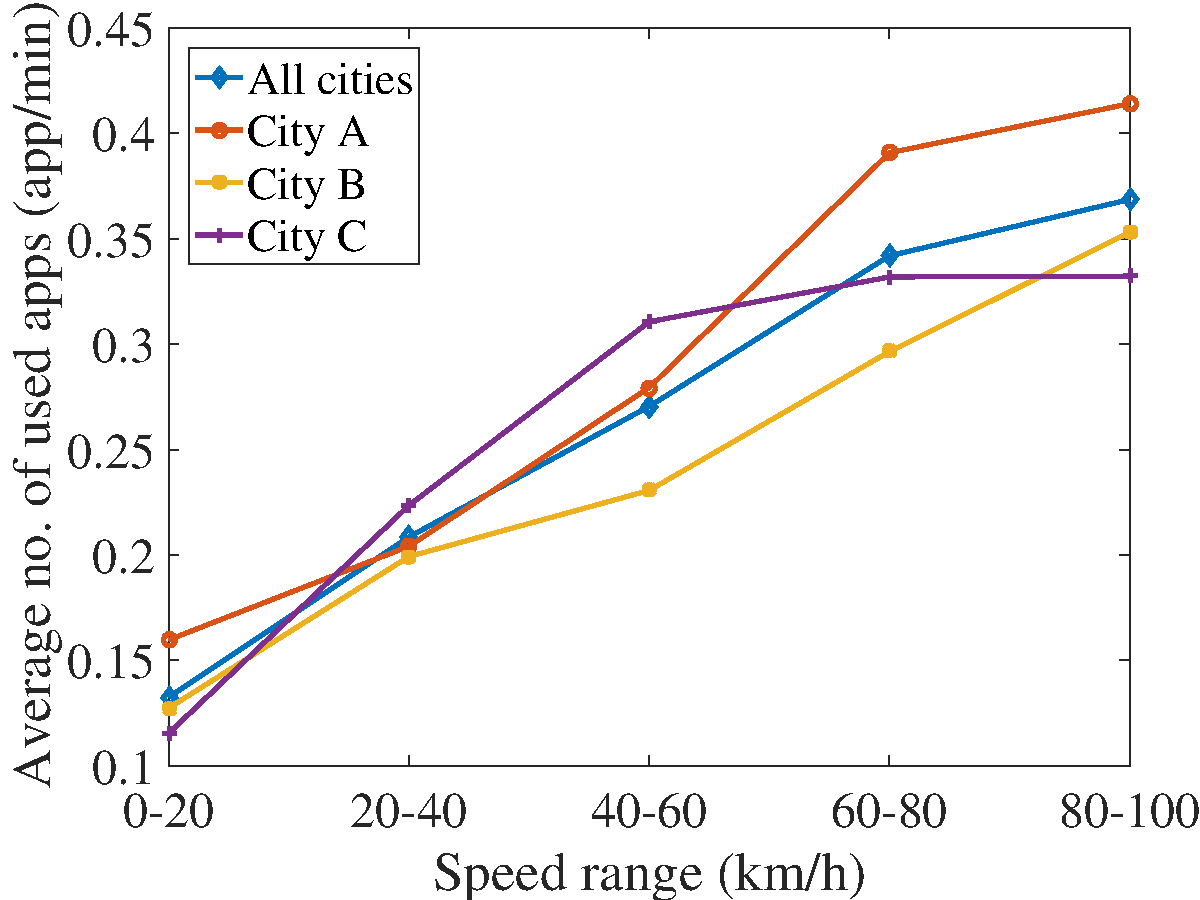
\includegraphics[width=0.32\linewidth]{./figures/large_font/speed_diversity.pdf}}
    \vspace{-0.1in}
    \caption{The (a) speed estimates; and its correlation with (b) data volume, (c) average time interval between consecutive data access, (d) time interval between consecutive connections, (e) average data access volume for each data access and (f) average number of apps used.}
    \label{fig:speed_corr}
\end{figure*}

With our methodology on speed estimates, we next explain our findings on correlations between user mobility and mobile data access patterns in this section. We start with the correlation of the speed and the average mobile data access volumes. Then we reveal the relation of speed and average time intervals between consecutive mobile data accesses. Finally, we illustrate the correlation between speed and the types of app usage that are responsible for generating the corresponding mobile data traffic.

\subsection{Experiment Settings}

To estimate the speed, our algorithm requires a user has visited at least 3 towers consecutively. In the dataset, we find that around 13 million records out of 58 million records can be utilized. In our experiments, to balance the accuracy of speed estimates and the number of mobile data access records that have qualified speed estimates, we set the threshold of both distance ratio $d_{ratio}$ and duration ratio $\Delta t_{ratio}$ empirically as 0.6. After the filtering, we have around 1 million records out of total 13 million records that meet both criteria. \autoref{fig:speed_cdf} shows the cumulative density function (CDF) of both raw speed estimates without filtering and filtered speed estimates. As we can see that the filtered speed estimates are more realistic compared to raw speed estimates. Most of the false high speed estimates and low speed estimates are filtered out by setting thresholds of confidence levels for distance estimates and travel time estimates.

%\begin{figure}[h]
    %\centering
    %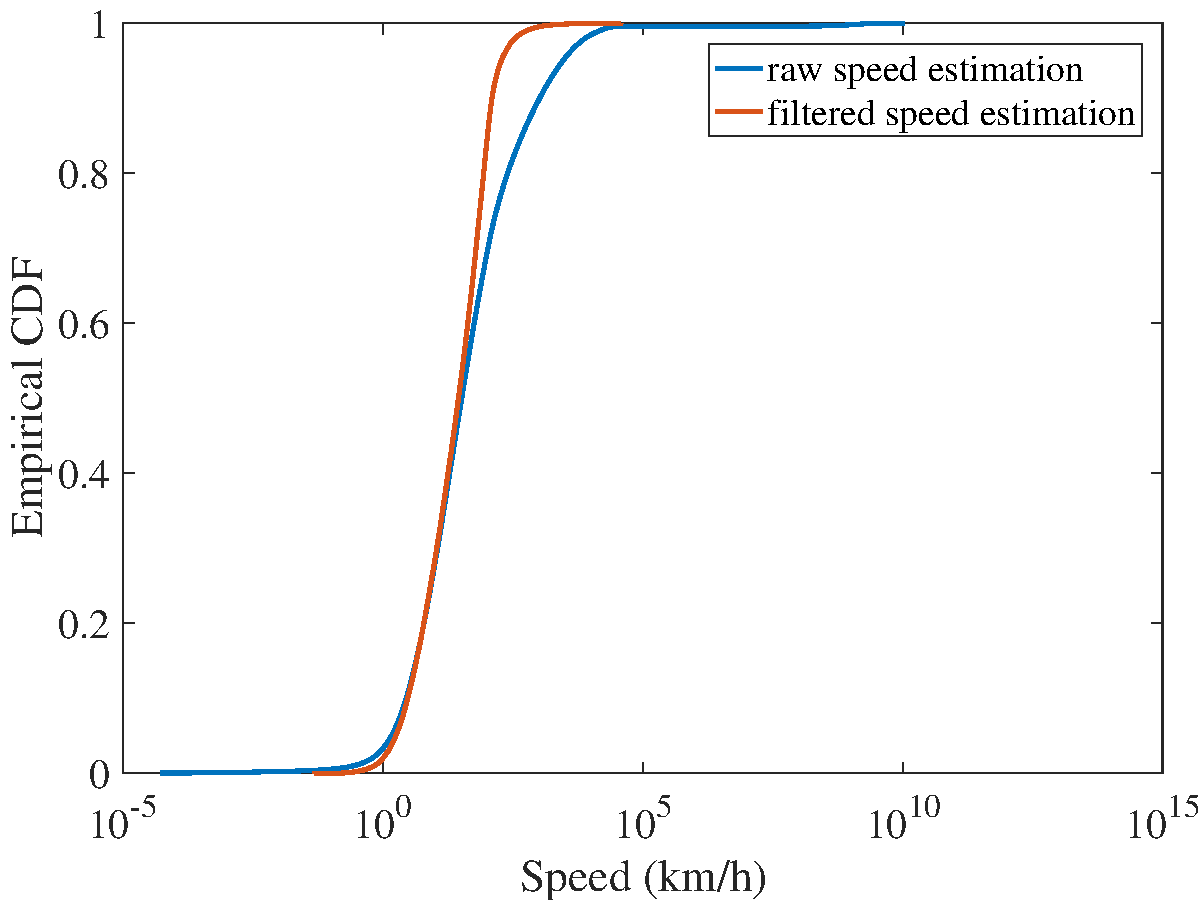
\includegraphics[width=\linewidth]{./figures/speed_cdf.pdf}
    %\vspace{-0.3in}
    %\caption{Empirical CDF of speed estimates.}
    %\label{fig:speed_cdf}
%\end{figure}

In the following experiments, we only show results in the speed range from 0 km/h to 100 km/h, since there are very few records with a speed estimate above 100 km/h for any meaningful insights.

\subsection{Speed and Data Volumes}

%\begin{figure}[h]
    %\centering
    %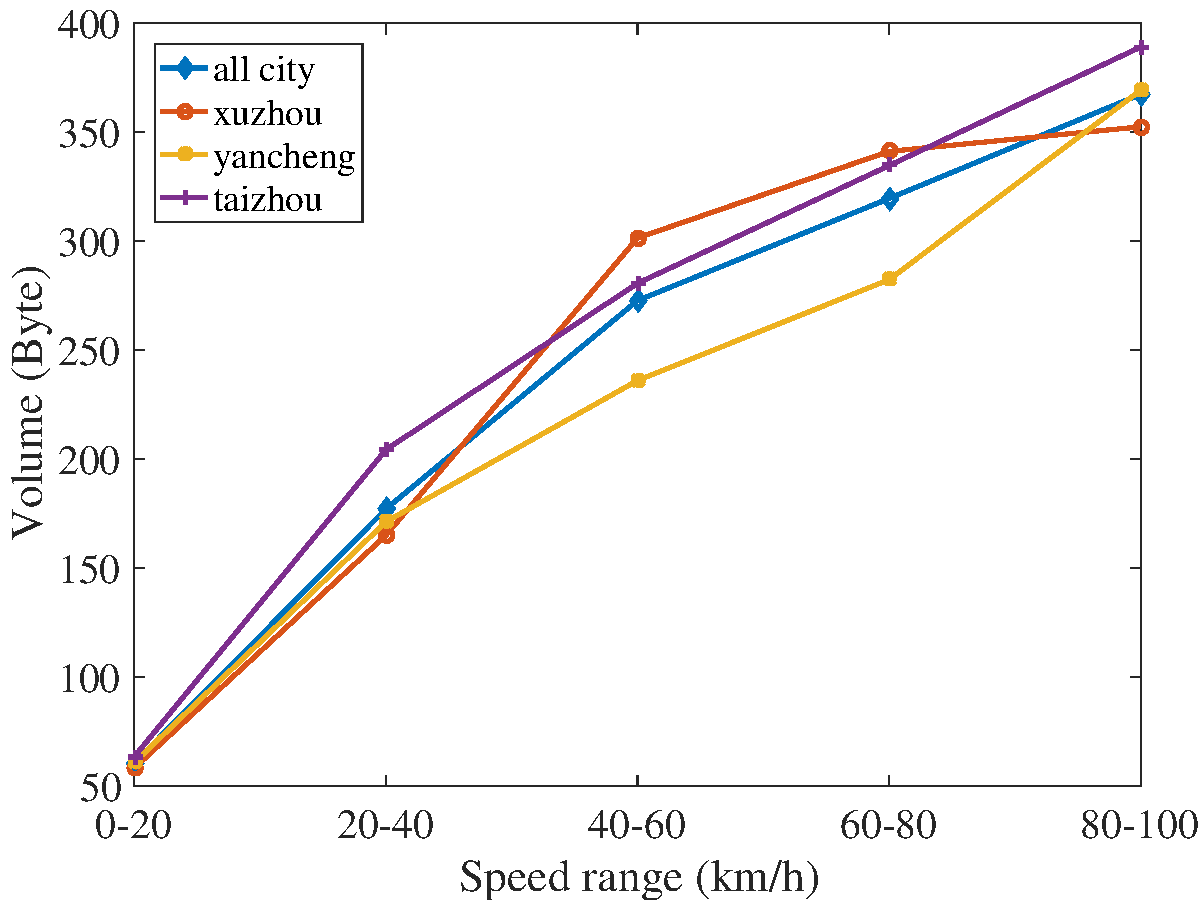
\includegraphics[width=\linewidth]{./figures/speed_vol.pdf}
    %\caption{Correlation between user speed and average access volume.}
    %\label{fig:speed_vol}
%\end{figure}

\autoref{fig:speed_vol} shows the results of the correlation of user speed and the average mobile data access volumes per user per second. We demonstrate the data from all three cities combined and each city respectively. The figure shows a clear trend that users are more active in accessing mobile data as the speed increases and the trend holds true for all three cities. In fact, a user with speed estimates of 80-100 km/h could reach an average data volume of 6 times of a low-speed user. Similarly, this trend also holds true for all the cities. Note that these results only show an increase in the mobile data access volume as user speed increases. It does not suggest lower speed users access online contents less frequently. Actually, we believe one reason might be that a large portion of a low-speed user's online needs is already fulfilled by various kind of high-speed connections such as Wifi hotspots. To this end, we reach similar findings with previous work~\cite{yang2015characterizing} on the correlation of user mobility and mobile data access volume, except that the previous work used the number of towers visited by a user as the indicator of user mobility.

\subsection{Speed and Access Frequency}

\begin{figure*}
    \centering
    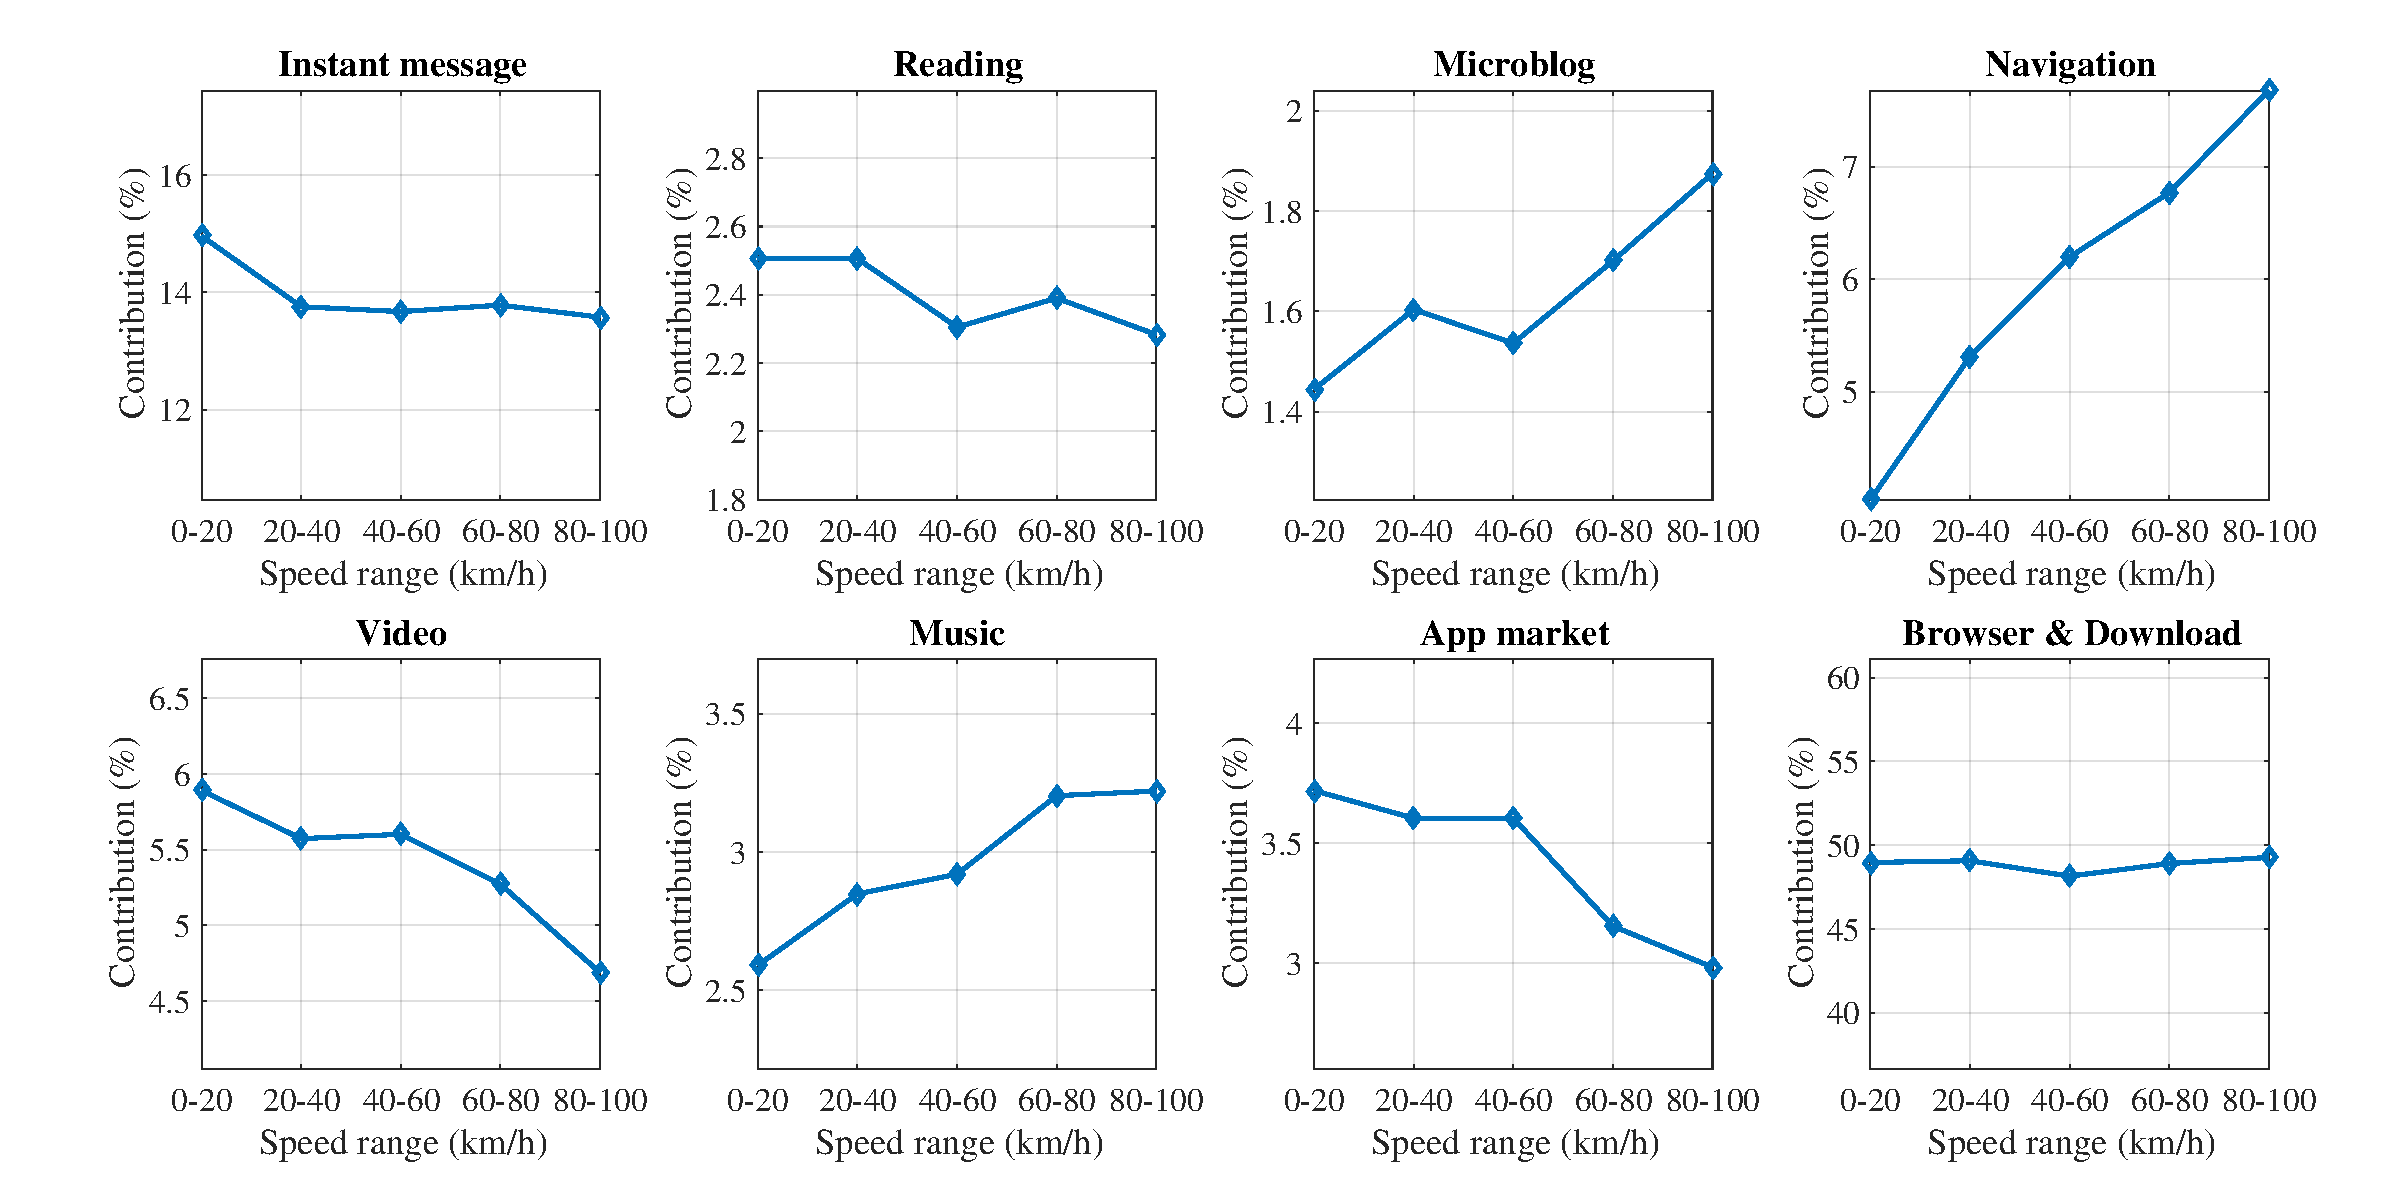
\includegraphics[width=\linewidth,height=3in]{./figures/large_font/speed_appcat.pdf}
    \vspace{-0.3in}
    \caption{Correlation of user speed and contribution of app categories.}
    \label{fig:speed_appcat}
\end{figure*}
%\begin{figure*}[h]
    %\centering
    %\subfigure[Average Time Interval\label{fig:speed_gap}]{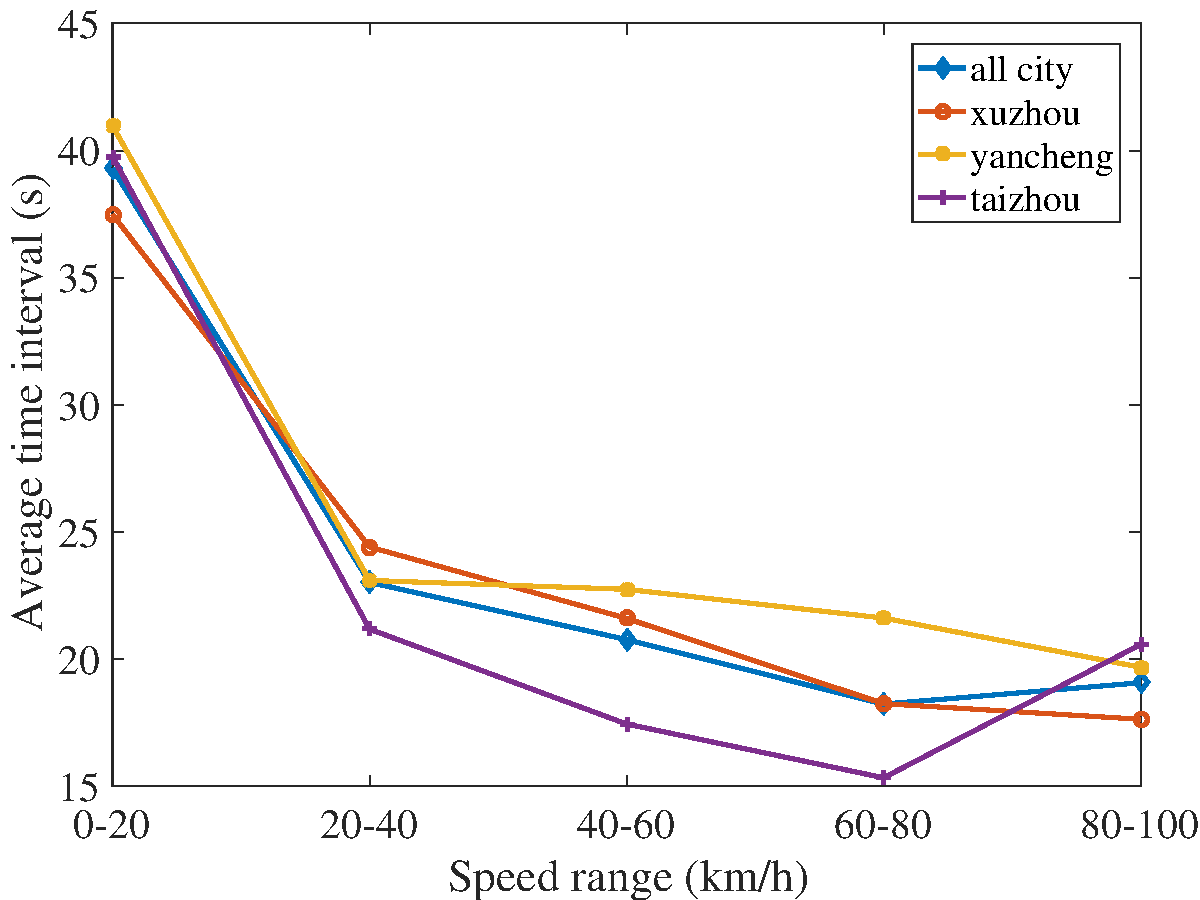
\includegraphics[width=0.32\linewidth]{./figures/speed_gap.pdf}}
		%\subfigure[Time Interval Empirical CDF\label{fig:speed_gap_cdf}]{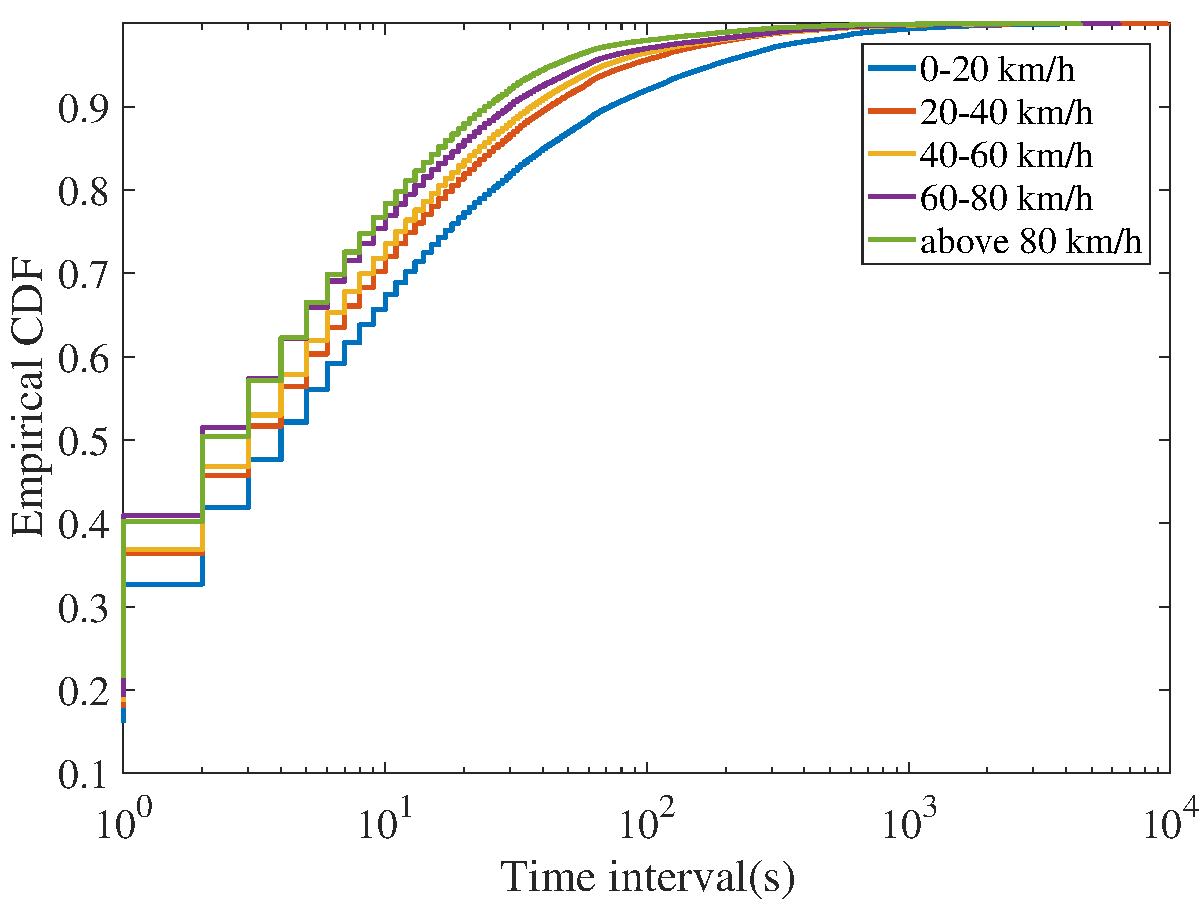
\includegraphics[width=0.32\linewidth]{./figures/speed_gap_cdf.pdf}}
		%\subfigure[Avearge volume per data access\label{fig:speed_per_conn_vol}]{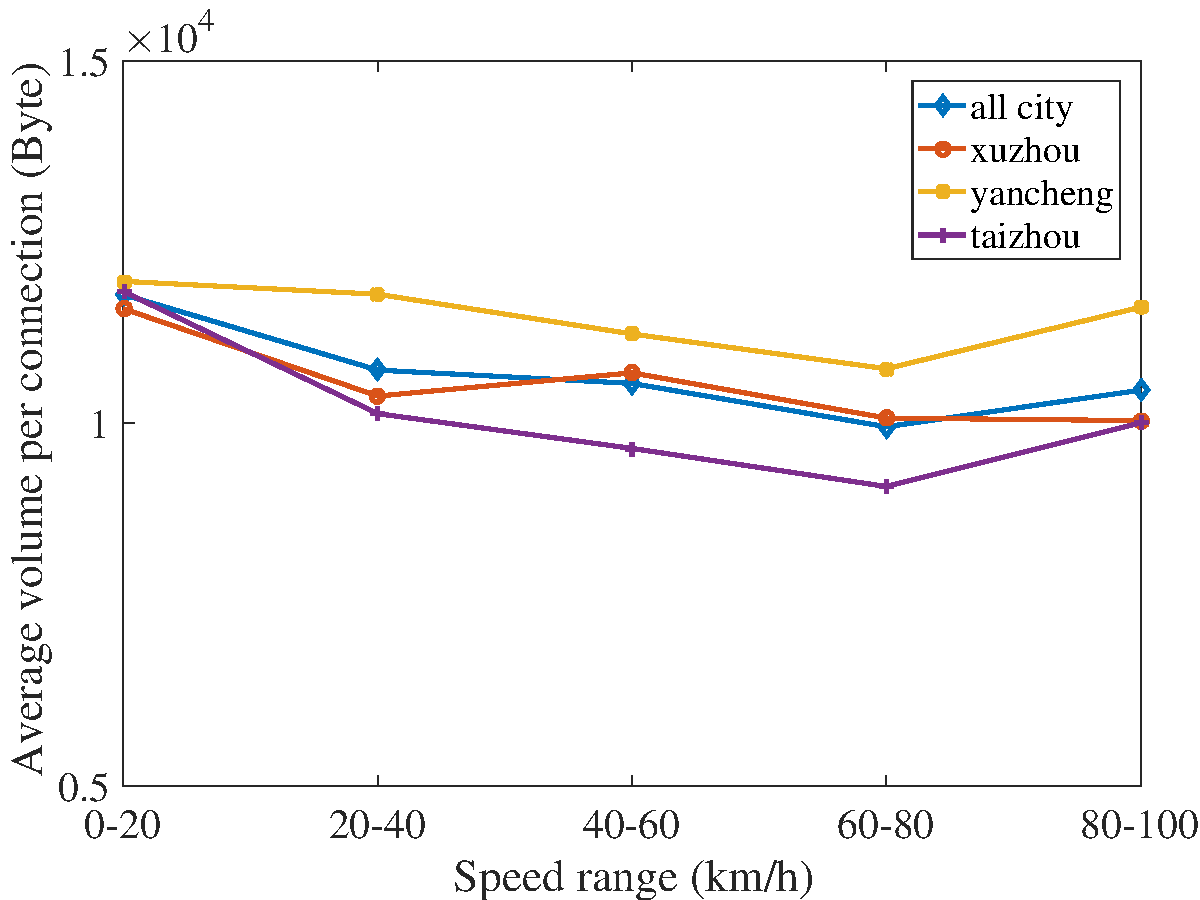
\includegraphics[width=0.32\linewidth]{./figures/speed_per_conn_vol.pdf}}
    %\vspace{-0.1in}
    %\caption{Correlation between user speed and (a) average time interval between consecutive data access, (b) Empirical CDF of time interval between consecutive connections and (c) average data access volume for each data acess}
    %\label{fig:speed_corr}
%\end{figure*}

%We show the correlation between user speed and mobile data access pattern in \autoref{fig:speed_corr}.
\autoref{fig:speed_gap} shows the correlation of speed and average time intervals between consecutive mobile data access records. The CDF of data time intervals for various speed ranges of all three cities are also shown in \autoref{fig:speed_gap_cdf}. Note that since the time precision of our data trace is seconds, so there are steps in \autoref{fig:speed_gap_cdf}. The decrease in time intervals as speed increases suggests that high-speed user accesses mobile data more frequently than low-speed users. A user with a speed estimate of 80-100 km/h access mobile data almost twice more frequently than a user with a speed estimate of 0-20 km/h on average. The trend holds for all three cities except that there is an odd point at 80-100 km/h for one city, which may be caused by the lacking of available data.

We show the average volume for each data access in \autoref{fig:speed_per_conn_vol}. As the user speed increases, there is no apparent correlation with average volume for each data access. This suggests that increasing in the average volume which is shown in \autoref{fig:speed_vol} is mainly cause by the increased data access frequency, not the volume for each data access.

\subsection{Speed and App Choice}

%\begin{figure}[t]
    %\centering
    %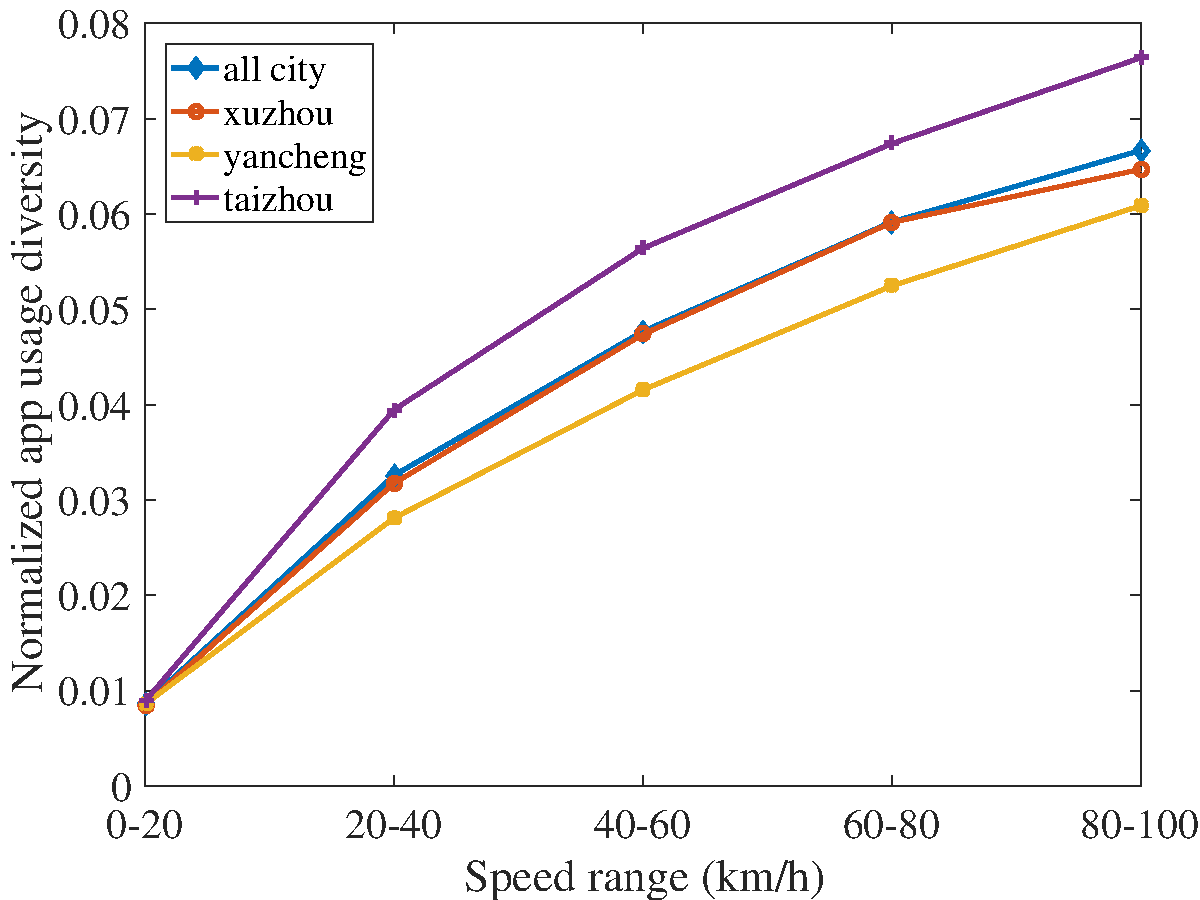
\includegraphics[width=\linewidth]{./figures/speed_diversity.pdf}
    %\vspace{-0.3in}
    %\caption{Correlation of user speed and normalized number of apps being used.}
    %\label{fig:speed_diversity}
%\end{figure}

%In this section, we first show in
\autoref{fig:speed_diversity} shows the correlation between user speed and the average number of apps being used for each user during each data segment per minute.
The trend clearly shows that as the speed goes up, the app usage diversity increases rapidly.
A user with a speed estimate of 80-100 km/h could use as many as 8 times apps per unit of time compared to a low-speed user.
This trend holds true for all the cities. An explanation might be that for users with high mobility, they may use their phones more often, switch between apps more, and be less likely to focus on one app for prolonged periods of time. 

%\subsubsection{App Category Information}

%In this section,
We further investigated the trend of the contribution of various app categories on the total mobile data access as the user speed increases.
The contribution was defined as the mobile data access of one category versus all categories.
According to the mobile service provider, each app in our dataset was assigned to one of 19 categories.
%However, the volume of data for each category is not even, among all 19 categories, we only interested in the
Focusing on apps that contributed the most to the total mobile data access volume,
we selected the top 8 app categories, as shown in \autoref{table:appcat}.
The correlation between the user speed and the contribution of each category is shown in \autoref{fig:speed_appcat}.
%Note that we do not show the correlation for each individual city because for some app categories there is not sufficient data to show a clear trend.

\begin{table}[h]
	\centering
	\begin{tabular}{lrr}\hline
	App Category & \# Apps & Volume (GB) \\
    \hline
	Instant Messages & 30 & 97.3\\
	Reading & 101 & 17.6\\
	Microblog & 43 & 13.0\\
	Navigation & 38 & 10.8\\
	Video & 63 & 45.2\\
	Music & 33 & 27.4\\
	App Market & 45 & 37.0\\
	%Game & 106 & 9.2\\
	%Online Payment & 18 & 1.2\\
	%Comic & 12 & 0.8\\
	%Email & 10 & 1.5\\
	%P2P & 8 & 3.9\\
	%VOIP & 17 & 0.3\\
	%Multimedia Messages & 2 & 0.3\\
	Browser \& Download & 558 & 353.5\\
	%Finance & 25 & 0.7\\
	%Security & 22 & 5.2\\
%	Other1 & 237 & 74.7\\
%	Other2 &   7 & 21.1\\
	Others & 464 & 118.9\\
    \hline
	\end{tabular}
	\caption{App categories}
	\label{table:appcat}
\end{table}

%\subsubsection{Impact of speed on each smartphone app category}

Among the top 8 categories, Microblog, Navigation and Music show a clear upward trend as the speed increases.
The impact of navigation has the most steady increase due to the increased needs for such apps when driving.
The impact almost doubles for users with speed estimates of 80-100 km/h compared to users with speed estimates of 0-20 km/h.
Instant message, Video and App market show a downward trend as the speed increases.
The reason could be the users are cost sensitive and strictly control the data usage for large app downloading and video streaming.
Browser \& Downloading and Reading show a quite stable impact that does not change a lot as the speed increases.

